\section{Approach}
\label{sec:model}
In this section, we describe our multi-task selected learning for solving the 3D-FBPP.
The overall architecture of our multi-task networks is shown in Figure \ref{fig:architecture-model}.
Basically, the procedure of solving the 3D-FBPP can be divided into three related tasks: sequence generation, orientation generation and spatial location selection. In order to leverage useful information contained in these multiple related tasks to help improve the generalization performance of all the tasks, we adopt a multi-task framework. Similar to classic 3D-BPP, which uses an empty-maximal-space representation to manage the spatial location in the bins, we fake a large enough bin to split the space and determine the spatial location. Figure \ref{fig:freespace} illustrates the concept of empty-maximal-space. However, among these tasks, the spatial location set is dynamic and hard to incorporate with the existing neural network. In this work, we disregard the spatial location selection strategy and greedily choose the empty-maximal-space according to least waste space criteria (LWSC), which aims to obtain least surface area at each step. 
\KZ{Did you invent LWSC? If so, you can say so. Otherwise, cite.}
LWSC, a simple greedy algorithm, inserts the node (item, orientation, spatial location) with least increased surface area to a partial solution and is problem-specific for our 3D-FBPP. For example, when placing items in the packing process, we choose the orientation and spatial location of increasing the minimum surface area by traversal. Therefore, we can concentrate on the sequence and orientation generation problems.  %Actually, the combination of results of 3D-FBPP is $6^{n}n!$ in case of not taking spatial location into consideration. To search that huge space in limited time is impossible, so that we'd better employ neural network to make decisions straightly.
\begin{figure}[h]
	\centering
	\epsfig{file=freespace.png, width=0.85\columnwidth}
	\caption{Example of empty-maximal-space. a) item packed in the bin ; b), c), d) newly generated maximal-spaces with the large fake bin, shown in yellow. }
	\label{fig:freespace}
	\vspace{-10pt}
\end{figure}

Sequence task is sequential decision problem, whereas the orientation task is a classification one. Since the two correlated tasks work together to benefit each other, we prefer to use a parameter-shared framework instead of training them separately. 
Recently, pointer network (Ptr) \cite{bahdanau2014neural}, whose output may be expressed as a sequence of indexes referring to elements of the input sequence, has been widely used to learn a heuristic algorithm for sequential decision problem like TSP. In this paper, we employ this architecture to tackle sequence task and add a softmax-layer to obtain classification-based orientation. Therefore, our 3D-FBPP solver is a multi-task encoder-decoder model based on Ptr.

%Nevertheless, unlike the original DRL-based Ptr model to solve combinational optimization problem \cite{bello2016neural} where the decoder cell will calculate the attentional distribution of inputs and only select one of them, we provide the sequence and orientation simultaneously.
Formally, a 3D-FBPP instance with $n$ items can be denoted as $\bi{x} = \{x_i=(l_i, w_i, h_i)\}_{i=1}^n$, where $l_i$, $w_i$ and $h_i$ represents the length, width and height of item $i$ respectively. The problem also features additional constraints, e.g, non-overlap, complicating the environment. The solution to this problem is a sequence of triplets $\{(s_i, o_i, f_i)\}_{i=1}^n$ which must meet these constraints, where $s_i$, $o_i$ and $f_i$ represent the item, orientation and spatial location to be placed in step $i$ during packing. Remarkably, $s_i$ and $o_i$ are produced by our model while $f_i$ is calculated by the greedy strategy LWSC mentioned above.  %We represent the packing sequence $\bi{s}={s_1,s_2,...,s_n}$ as a permutation of the items $\bi{x}$ . 
Our model reads the sequence of input tokens (items \bi{x}) with Long
Short-Term Memory (LSTM) [16] encoder and meanwhile decodes
the sequence of output tokens (items \bi{s} and orientation \bi{o}). During decoding steps, the input of decoder cell for time-step $i$ contains two parts denoted as $y_i=(s_i, o_i)$. Specially, the packing sequence $\bi{s} =\{s_1,s_2,...,s_n\}$ is a permutation of the input items $\bi{x}$. 
%In addition, the sequence and orientation tasks share the most of wights and the only difference exists in the output.%


\begin{figure}[h]
	\centering
	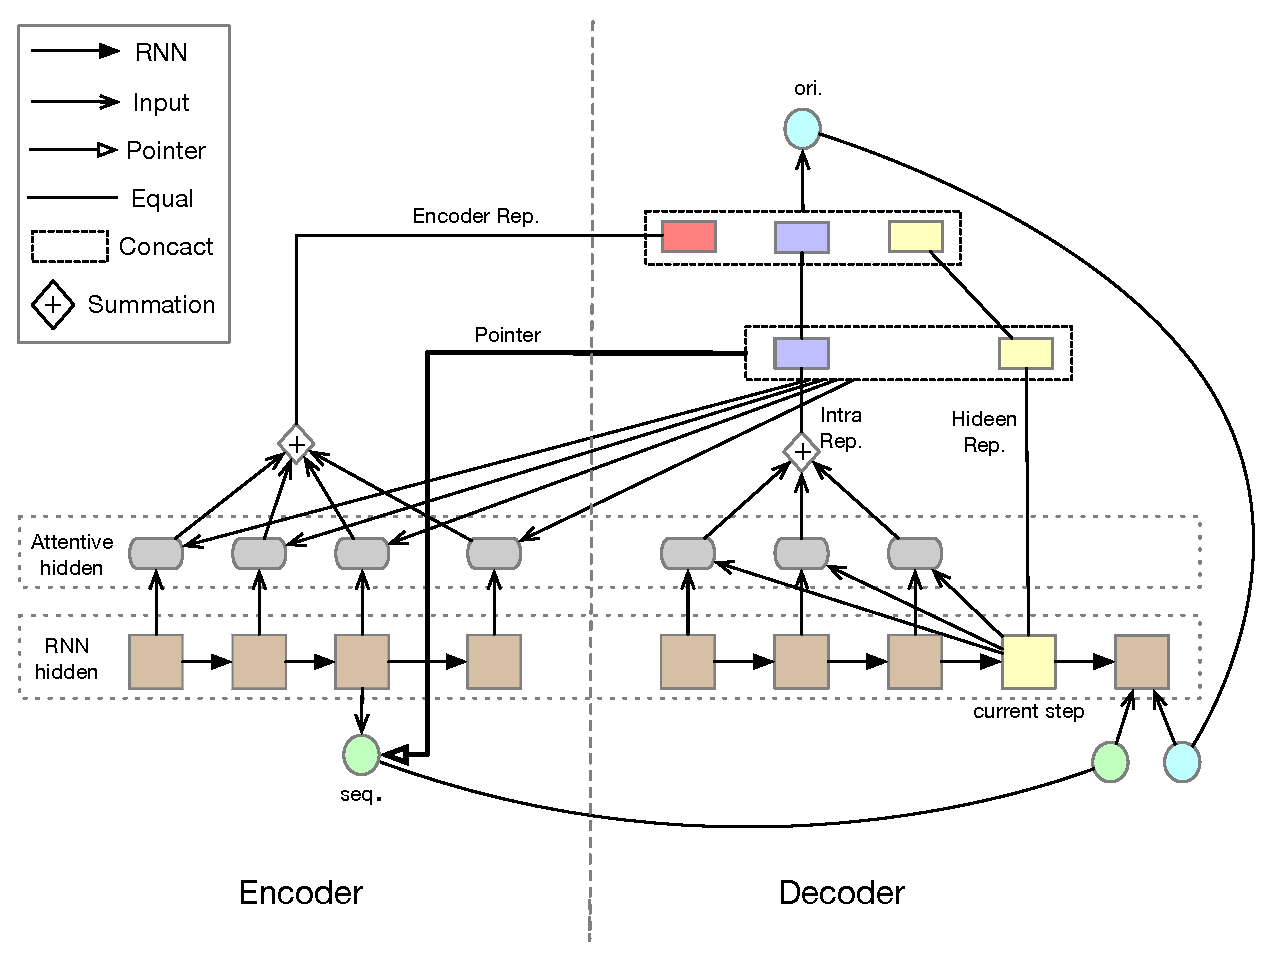
\epsfig{file=binpacking.eps, width=0.95\columnwidth}
	\caption{Architecture for multi-task 3D-FBPP networks. Rep.,ori. and seq. is short for representation, orientation output and sequence output, respectively. }
	\label{fig:architecture-model}
	\vspace{-10pt}
\end{figure}


\subsection{Sequence Task}
\label{sec:sequence_task}
Due to the particularity of the 3D-FBPP, it's not allowed to pack the same item repeatedly. The way to prevent the sequence from containing the same item 
twice in the previous work \cite{bahdanau2014neural} is a hard constraint and 
it seems that the information of the generated subsequence is independent of 
the probability distribution of next items.
%Even though this method has generated a better sequence to pack the items, it's unreasonable \yu{confused}.
Obviously, incorporating the information of previous decoding steps into the decoder can help us to generate more reasonable and structured pointers.   
Moreover, taking previously decoded items into consideration means that the network has a priori knowledge to try to avoid repetition to some extend.
To achieve this, we introduce an intra-attention mechanism \cite{paulus2017deep}, which is first proposed to solve the current combinational optimization problem. 

For notation purposes, let us define encoder and decoder hidden states as $h_{i}^{e}$ and $h_{t}^{d}$ respectively. 
Here $h_{i}^{e}$ and $h_{t}^{d}$ are computing from the embedding vector of $x_{i}$ and $y_{t}$ respectively.
We define $attn_{tj}^{d}$ as the intra-attention weight of the previous hidden states $h_{j}^{d}$ at decoding step $t$:
\begin{eqnarray*}\label{1}
	&attn_{tj}^{d} = softmax(v^{T}tanh(W_{1}h_{j}^{d} + W_{2}h_{t}^{d})),\\& j \in \{1,\dots,t-1\},
\end{eqnarray*}
where $W_{1}$, $W_{2}$ and $v$ are trainable parameters for intra-attention.
Thus, the intra-attention feature $h^{intra}_{t}$ of the current decoding item $s_{t}$ is calculated by summing up the previous decoded hidden states based on the computed intra-attention weights, for $t > 1$: 
\begin{eqnarray*}\label{2}
	&h^{intra}_{t} = \sum_{j=1}^{t-1}{attn_{tj}^{d}h_{j}^{d}},	
\end{eqnarray*}
Especially for the first decoder cell, we set $h^{intra}_{1}$ to a vector of zeros since the already generated sequence is empty.

In previous deep reinforcement learning (DRL) method for combinatorial optimization problems, the pointer mechanism considers the encoder attention weights as the probability distribution to copy the input item. In this work, we get the final attention weights $p(s_{t})$ by integrating intra-attention feature at decoder step. In addition, $u_j^t$ is intermediate result which will be normalized by softmax to be the ``attention'' mask over the inputs. 
\begin{eqnarray*}\label{3}
	%	\begin{array}{m}
	&u_{j}^{t} = {v^{'}}^{T}tanh(W_{3}h_{j}^{e} + W_{4}h_{t}^{d} + W_{5}h^{intra}_{t}) \nonumber, \\
	&p(s_{t}) = softmax(u^{t}), \quad j\in\{1,2,...,n\},	 %\eqno(3)   
	%	 \end{array}
\end{eqnarray*}
where $W_{3}$, $W_{4}$, $W_{5}$ and $v^{'}$ are trainable parameters for pointer networks.
We refer all parameters for sequence task as $\theta_{seq}$ and the probability distribution output of sequence task as $p_{\theta_{seq}}(\cdot|\bi{x})$ in the following discussions.

\subsection{Orientation Task}
When stacking a cuboid-shaped item, there are 6 orientations, for which we have 3 choices in the first dimension and 2 in the second. For 3D-FBPP, these 6 kinds of orientations are defined as: front-up, front-down, side-up, side-down, bottom-up and bottom-down. For orientation generation, the decoder computes the orientation based on a context vector $\bi{c}$,
which describes the whole problem and is based on the partial solution constructed so far. That is the context of the decoder at time step $t$ comes from the encoder outputs and the outputs up to time step $t$. For each time step $t$, we calculate the context vector:
\begin{eqnarray*}\label{4}
 	c_t = [h^{e};h_{t}^{d};h^{intra}_{t}].
\end{eqnarray*}
Here, [.;.;] denotes vector concatenation,
$h^{e}$ donates the representation of input sequence and is calculate by an attention-polling function which is defined as follows:
\begin{eqnarray*}
	&h^{e} = \sum_{j=1}^{n}{att_{tj}^{d} * h_{j}^e}, \\
	&attn_{tj}^{d} = softmax({v^{''}}^{T}tanh(W_{6}h_{j}^{e} + W_{7}{[h_{t}^{d};h^{intra}_{t}]})), \\
	& j \in \{1,\dots,n\}.
\end{eqnarray*}
Where $W_{6}$, $W_{7}$ and $v^{''}$ are trainable parameters for attention-polling function.
And we apply the intra-attention feature $h^{intra}_{t}$ similar to the previous section to represent the context up to current decoding step $t$.

Thus, the probability distribution of orientations for the current decoding step $t$ is generated by as follows:
\begin{eqnarray*}\label{5}
	p(o_{t}) = softmax(W_{ori}c_t + b_{ori}),
\end{eqnarray*}
where $W_{ori}$ and $b_{ori}$ are trainable parameters for orientations.

We define $\bi{o}^{*} = \{o_{1}^{*},o_{2}^{*}, ..., o_{n}^{*}\}$ as the ground-truth orientation sequence for a given input $\bi{x}$ and generated packing item sequence $\bi{s}$. As a matter of fact, $\bi{o}^{*}$ is calculated greedily according to LWSC, using the item placement sequence generated by our sequence task mentioned above. At each step, we will exhaustively search all possibilities of given spatial locations and orientations to find the one with least surface area for the current item.  

As we apply supervised training in this part, the objective is to maximize the likelihood of all orientation labels $\bi{o}^{*}$, given the partially generated placement sequence $\bi{s}^{'}$ and model parameters $\theta_{ori}$ for orientation task:
\begin{eqnarray*}
	\log{p(\bi{o}^{*}|\bi{s}^{'}, \theta_{ori})} = \sum_{i=1}^{n}\log{p(o_{i}^{*}|s_{1}, o_{1}^{*},..., s_{i}, \theta_{ori}, \bi{x})}.
\end{eqnarray*}

Besides, We refer the probability distribution output of orientation task as $p_{\theta_{ori}}(\cdot|\bi{x})$ in the following discussions.

\subsection{Training and Testing}
\label{sec:training_Testing}
In this subsection, we will illustrate the training and testing procedure which is specially designed for the 3D-FBPP.
\subsubsection{Training}
\label{sec:train}

To train a multi-task model, we use a hybrid loss function to combine supervised learning and reinforcement learning.
For sequence task, we use a well-known policy gradient approach named REINFORCE \cite{williams1992simple}. However, for orientation task, the orientation is chosen stochastically from a distribution parameterized by supervised learning. Nevertheless, as the orientation task is much more complex, the sequence task will suffer from the bad initializer of orientation if they are trained at the same time. To overcome this shortcoming, pre-training the orientation task first could be a reasonable idea.
However, orientations of the items is tightly attached to the existence of packing sequence of items in the 3D-FBPP. 
Consequently, as a trade-off, we train different types of tasks separately for each batch to keep them dynamically balanced.
We called this \textbf{M}ulti-\textbf{t}ask \textbf{S}elected \textbf{L}earning (MTSL). Mathematically, there are three kinds of basic loss function in our work:
\begin{eqnarray*}
	%\begin{array}{m}
	&p_{\theta_{seq}}(s_{i}|\bi{x}) = {p(s_{i}|s_{1},o_{1}^{*}, ..., s_{i-1}, o_{i-1}^{*}, \bi{x})},\\
	&L_{seq} = (SA(\bi{s},\bi{o}|\bi{x}) - bl(\bi{x}))\sum\limits_{i=1}^{n}\log{p_{\theta_{seq}}(s_{i}|\bi{x})},\\
	&p_{\theta_{ori}}(o_{i}^*|\bi{x}) = {p(o_{i}^*|s_{1},o_{1}^{*}, ..., s_{i-1}, o_{i-1}^{*}, \bi{x})},\\
	&L_{ori} = -\sum\limits_{i=1}^{n}\log{p_{\theta_{ori}}(o_{i}^*|\bi{x})},\\
	&L_{all}  = L_{seq} + L_{ori},
	%\end{array}
\end{eqnarray*}
where $SA(\bi{s},\bi{o}|\bi{x})$ denotes the surface area of the bin in the case of 
placement sequence and its corresponding orientation of $\bi{o}$ and $\bi{s}$, 
and $bl(\bi{x})$ denotes the baseline surface area initialized by LWSC. During training, to relief the correlation and imbalance, our model will choose one of the three kinds of loss $\{L_{seq}, L_{ori}, L_{all}\}$ according to a probability distribution which will decay after several training step.  

For sequence task, as we use the REINFORCE estimator with baseline, a good baseline can reduce the variance of the estimator and facilitate our learning. In this work, we resort an exponential moving average baseline as there is no need to differentiate between inputs and simple to implement, rather than critic \cite{degris2012off-policy}. For an sample $\bi{x}$, the baseline value is updated as $bl(\bi{x}) = SA(\bi{s},\bi{o}|\bi{x})+\alpha(bl'(\bi{x})-SA(\bi{s},\bi{o}|\bi{x}))$ with a decay $\alpha$.

As a conclusion of the discussion above, the training procedure of our Multi-task Selected Learning method can be summarized in Algorithm \ref{alg-summary-drl}.

\begin{algorithm}                  % enter the algorithm environment
	\caption{Multi-task Selected Learning.}       
	\label{alg-summary-drl} 
	\begin{algorithmic}[1]
		\State Training set $X$, training steps $T$, batch size $B$.
		\State Init. Sequence and Orientation parameters $\theta_{seq}$, $\theta_{ori}$.
		\State Init. baseline value $bl$ according to LWSC.
		\For {\emph{t = 1 to T}}
		\State Select a batch of samples $\bi{x}$, calculate baseline $bl(\bi{x})$.
		\State Sample solution $\bi{s}$ by sequence prob. $p_{\theta_{seq}}(\cdot|\bi{x})$.
		\State Obtain spatial location $\bi{f}$ and orientation $\bi{o}^{*}$ for $\bi{s}$ by LWSC.
		\State Calculate $SA(\bi{s},\bi{o}^{*}|\bi{x})$ by tuple $(\bi{s},\bi{o}^{*},\bi{f})$
		\State %$g_{\theta_{seq}}=\frac{1}{B}\sum\limits_{k=1}^{B}\nabla_{\theta_{seq}}\log{p(s_{t,k}|s_{t,1},o_{t,1}^{*},\dots,s_{t,k-1},o_{t,k-1}^{*},x_t)}*(SA(s_t, o_{t}^{*}|x_t)-bl(x_t)) $
		$g_{\theta_{seq}}=\mathbb{E}[(SA(\bi{s}, \bi{o}^{*}|\bi{x})-bl(\bi{x}))\nabla_{\theta_{seq}}\log{p(\bi{s}|\bi{x})}]$
		\State  %$g_{\theta_{ori}}=\frac{1}{B}\sum\limits_{k=1}^{B}\nabla_{\theta_{ori}}\log{p(o_{k}^{*}|s_{t,1},o_{t,1}^{*},\dots,s_{t,k-1},o_{t,k-1}^{*},x_t)}$
		$g_{\theta_{ori}}=\mathbb{E}[\nabla_{\theta_{ori}}\log{p(\bi{o}^{*}|\bi{x})}]$
		\State 	$g_{\theta_{all}}= g_{\theta_{seq}}+g_{\theta_{ori}}$.
		\State  $g_{\theta} = choice(g_{\theta_{seq}},g_{\theta_{ori}},g_{\theta_{all}})$
		\State Update $\theta = ADAM(\theta, g_{\theta})$.
		\State Update baseline $bl(\bi{x}) = SA(\bi{s},\bi{o}^{*}|\bi{x}) + \alpha(bl'(\bi{x})-SA(\bi{s},\bi{o}^{*}|\bi{x}))$.
		\EndFor
		\State return all parameters $\theta_{seq}$, $\theta_{ori}$.
	\end{algorithmic}

\end{algorithm}


\subsubsection{Testing}
\label{sec:test}

Moreover, different from traditional machine learning problems, combinational optimization problems are to minimize or maximize the objective under a given set of constraints, which seems to have some of priori knowledge about how to evaluate the result. For the 3D-FBPP, the benchmark is the smaller the better. As evaluating a surface area is inexpensive, we can simply generate multiple candidate solutions per order at inference time and select the best. The way to generate candidates is based on the calculated probability $p_{\theta_{seq}}(\cdot|\bi{x})$ and $p_{\theta_{ori}}(\cdot|\bi{x})$. At inference time, in order to calculate the surface area, we firstly obtain the packing sequence and orientation by trained model, then greedily compute the spatial location according to LWSC. %Besides, the same procedure training and testing This harmonizes learning with the inference procedure, and lowers the variance of the gradients, improving the training procedure.  

